\chapter{The Eclipse IDE}\label{cha:TheEclipseIDE}

In the following chapter a general overview of Eclipse framework and its most prominent components is provided. A description and analysis of available plug-ins from which essential information could be captured is presented. Last but not least a great amount of focus is given on a specific plug-in which is used and enhanced throughout the thesis.  

%\todo{ide eclipse plug-ins, available what are useful, present all, write adv and dis. describe contextual factors that can be achieved, describe how programmers work within this ide. }
%\todo{focus on rabbit specia chapter explain why to choose that, positive negative, limitations. provide class diagram and explanation, name the issues}

\section{Eclipse}
\label{sec:TheEclipseIDE:eclipse}
Eclipse framework is an IDE fairly used by several developers: to primarily develop Java applications, to also develop in other programming languages via plug-ins, and to develop documents and packages for other softwares.

The standard SDK Eclipse distribution contains a base workspace with certain functionalities, Java Developemnt tooling plug-ins and layout. Thereafter additional plug-ins allow the extension of the workspace, and Eclipse can become a multifunction framework to be used for: 
Embedded programming, C++ programming, javaBeans, Java application, 
websites, or even develop additional Eclipse plug-ins, etc. 
The plug-ins can be removed or replaced according to the needs 
of the developer.

Even though Eclipse framework started as a replacement for Visual Age for Java from IBM% \todo{give reference},
it became an open platform for integrating tools, editors, views and plug-ins. 
Its source code is freely available and anyone can contribute by building their own 
new plug-ins or by engaging in discussions regarding integrated tools.  

\section{Menus, views and editors}

When starting up Eclipse, if its a newly initiated greets the developer with a welcoming screen, otherwise the previously work space is loaded. 
Figure \ref{fig:eclipse_worspace} displays a standard Eclipse setup, 
a java integrated development environment. Eclipse's main window is called as the \textit{workbench} and based on the active \textit{perspective} its appearance is defined. 
A perspective has its own a set of elements views and editors and menus along with a adaptable personalized layout for specific tasks such as debugging a 
program. 
\label{sec:TheEclipseIDE:menusviewsandeditors}
	\begin{figure}[!ht]
		\begin{center}
		 
        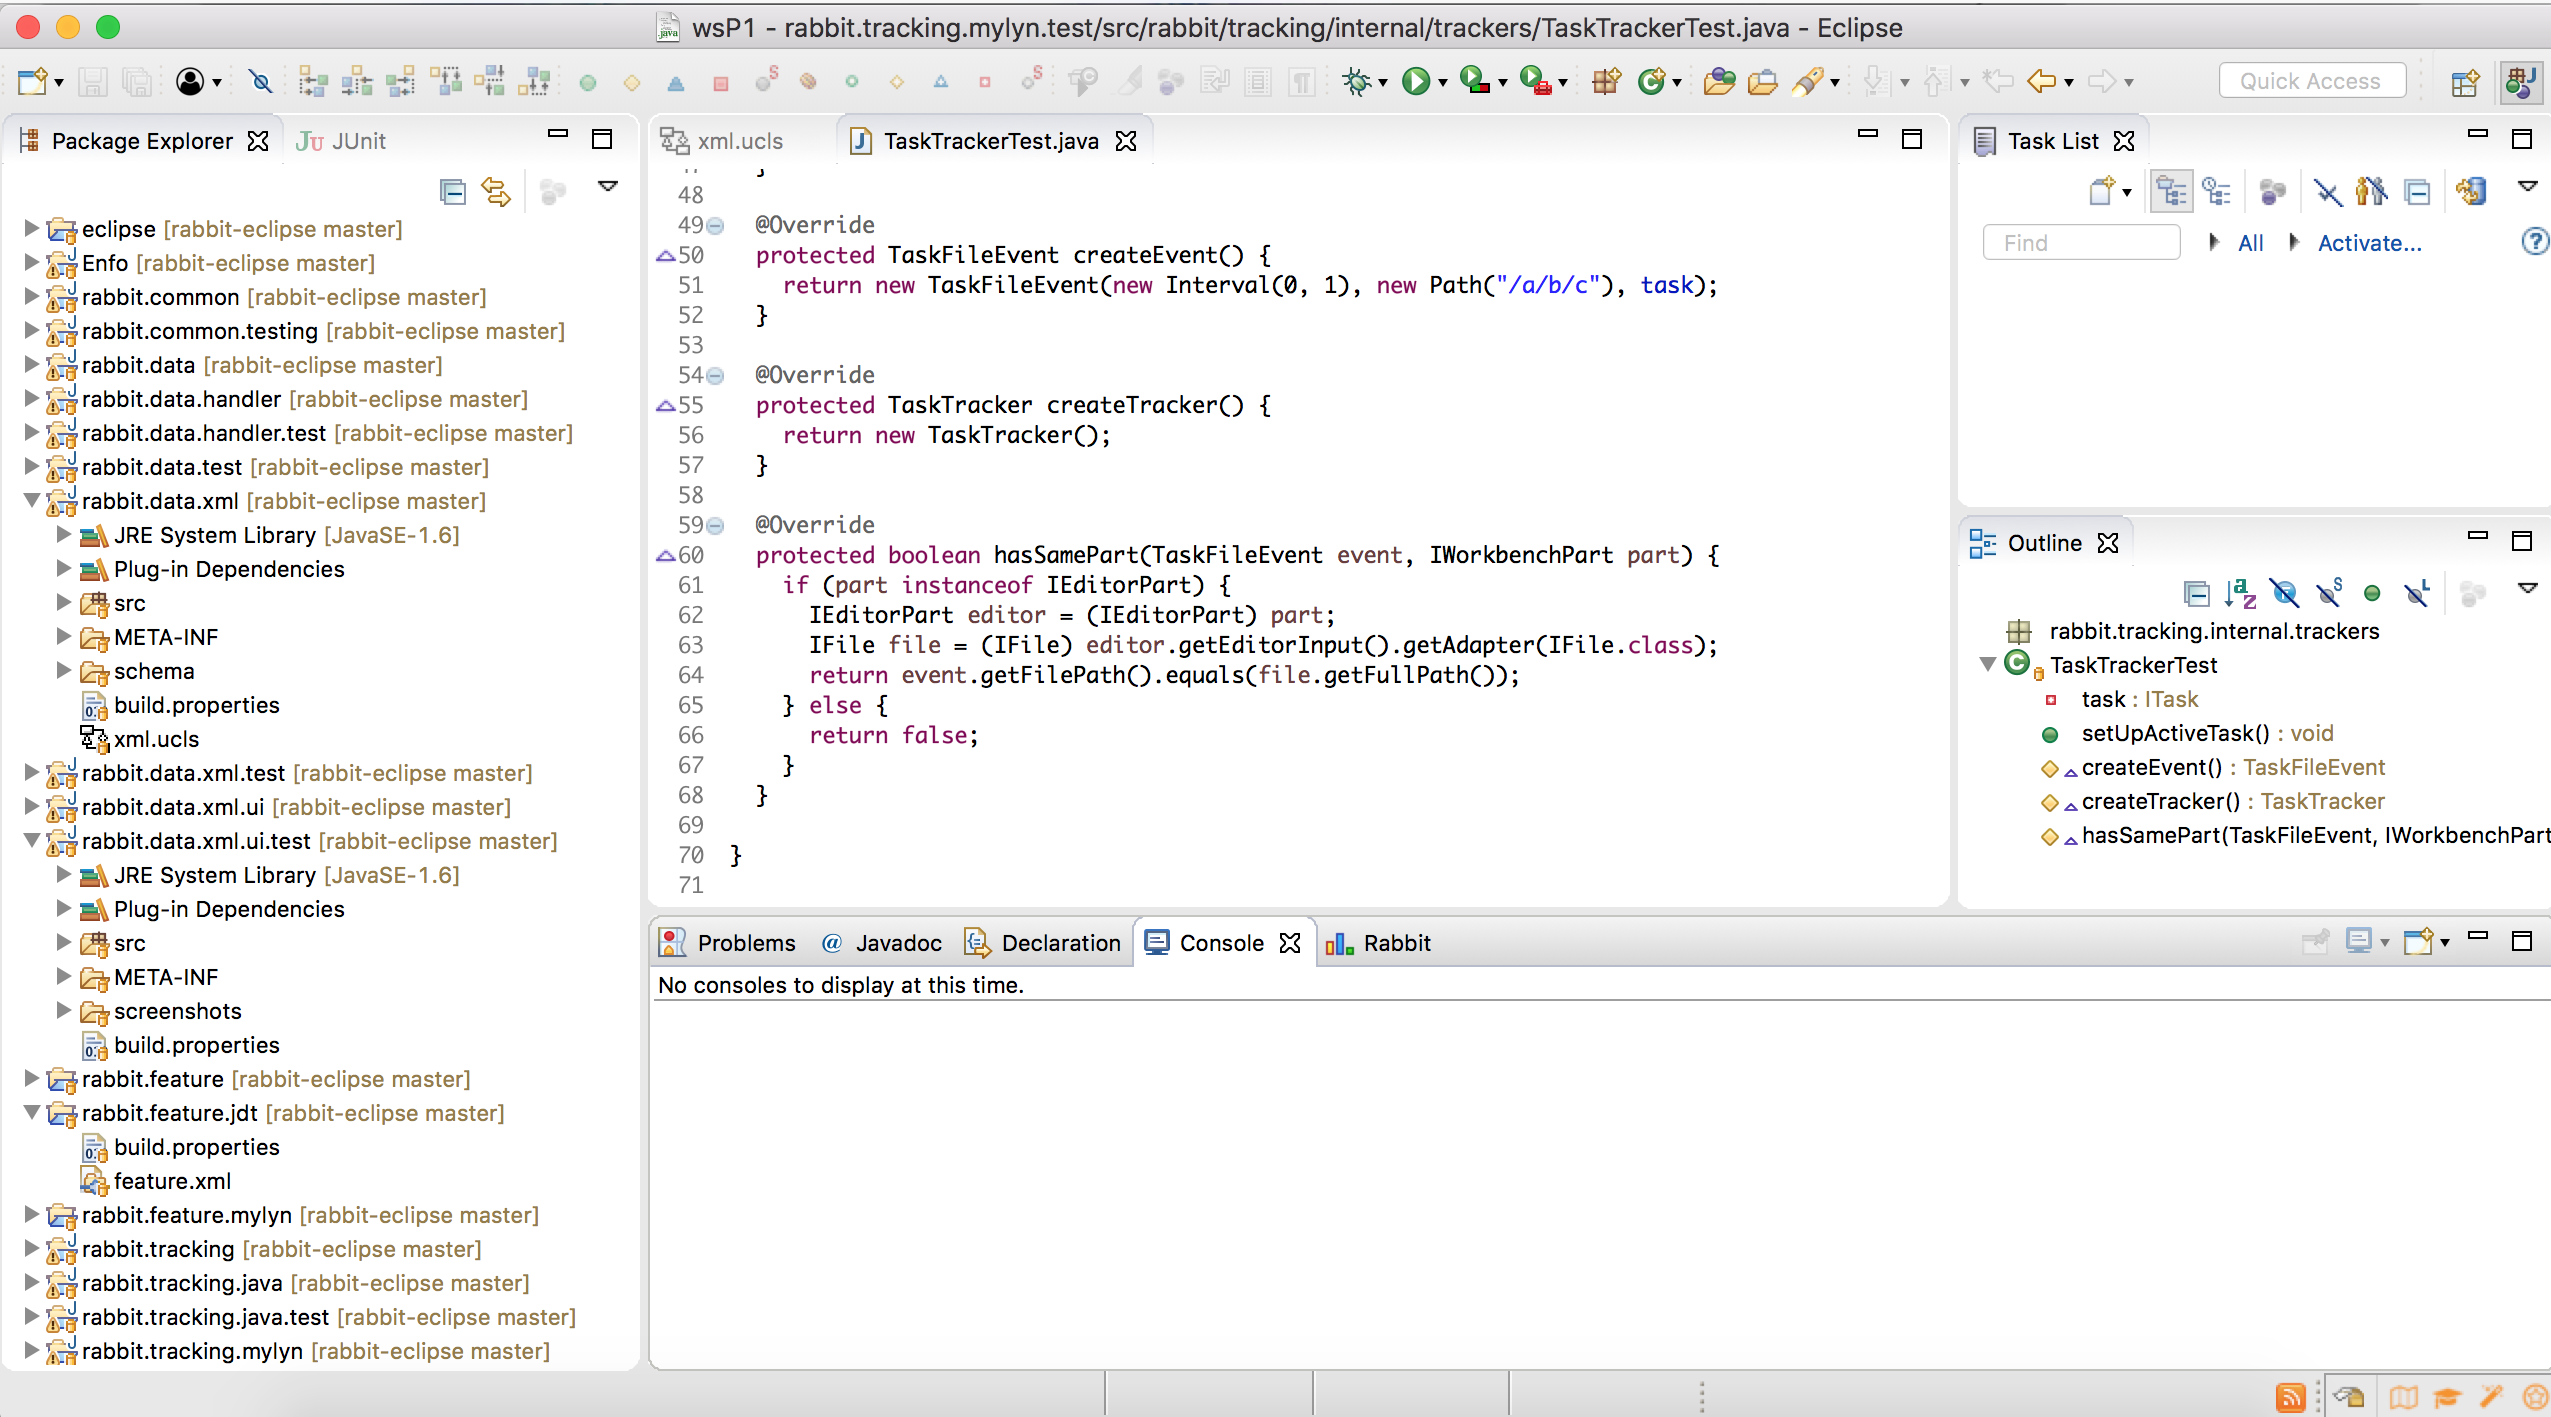
\includegraphics[width=\textwidth]{figures/eclipse_workspace.png}
		\end{center}
		\caption{The Java Development perspective in Eclipse.}
		\label{fig:eclipse_workspace}
	\end{figure}
A view is a window that enables the developer to examine something, eclipse offers various of views f.x. Java packages and their files.
An editor is a smart editor which recognizes the programming language markups the syntax and allows you to modify and save files. 
Editors share characteristics with views, but unlike views, editors don't have tool-bars.
Eclipse is filled up with menus and tool-bars, the main menu is at the top of the screen while views and explorers usually provide their own context menus.
Eclipse IDE is highly adjustable and enables the developer to construct and save his own perspectives building up his work space.



\section{Plug-ins}
\label{sec:TheEclipseIDE:plug-ins}
Eclipse is a multifunction framework and it provides several software components (plug-ins).
Eclipse Marketplace client gives the advantage of searching, and discovering popular extensions to developers enhancing their working environment.
These software components are usually distributed as \textit{jar} files. 
The Plug-in Developer Environment (PDE) enables developers to extend their Eclipse IDE by creating new additional functionalities 
or even improve the capabilities of already implemented plug-ins. 

Although the reason Eclipse provides this thumping range of tools is to support 
developers, usually instead a chaotic environment is generated. 
For this reason several researchers and developers instrumented plug-ins. There aim was to firstly 
understand developers' activity within an IDE, to evaluate the quality of code produced within an IDE 
and also to develop Recommendation system in software engineers (RSSEs). 

For this thesis the plug-ins in concern are mostly observing the usage of Eclipse artifacts and 
recording activity as well as interactions of a developer. 
Several of these type of plug-ins can be found in git-hub and the Eclipse Market, emphasize was given
to the following plug-ins:

\textbf{Fluorite} is a plug-in developed in the School of Computer Science 
at Carnegie Mellon university. Its purpose is low level event logging 
for Eclipse when using the code editor. In other words, events such as: 
%\todo{add link http://www.cs.cmu.edu/~fluorite/} 
character type, text cursor movement, 
selected text modification, as well as, all
the other available Eclipse commands that can be called for an editor.
Fluorite could potentially be used to extract developers' coding 
activity and use to detect and measure the time for various usage 
patterns or events of interest. However, this plug-in seemed promising 
and a good candidate for process mining, it was not possible to gain 
access to its source code.
 
\textbf{Usage Data collector} is a framework for collecting information about how developers 
are using the eclipse platform. Information for views usage, editor usage, 
changes of perspectives, actions invoked are recorder by monitors which
are being used including also a timestamp. Moreover this plug-in also collects 
basic information about the runtime environment (OS, system architecture, window system, 
locale, etc). This information are uploaded periodically to servers hosted by The Eclipse 
Foundation with the purpose to be processed in a later stage %\todo{https://www.eclipse.org/org/usagedata/}.
Since this plug-in records relevant information it could offer a useful structure for mining the developers workflow, 
however, due to the fact that the development stopped a long time ago, access to source code was not achieved.
The project was shut down mainly due to resource constraints. Despite the efforts of researchers, not valuable 
knowledge was obtained from the data. 
%\todo{however access to some data collected can be found and maybe is possible to do some process mining on those data}

\textbf{Metrics} is a plug-in that calculates various metrics for your code during build cycles and warns you of range violations for each metric.
%\todo{https://marketplace.eclipse.org/content/eclipse-metrics}. 
Metrics examples are the number of classes, children, interfaces, depth of inheritance, overridden methods,etc.
This information can be extracted as an xml and therefore some data mining could be performed.

\textbf{Mylyn} is a subsystem in Eclipse used for task management. The original name of this project is Mylar, and was used in studies such as %\todo{how are java softwaere developers usingthe eclipse IDE}
because it captures events, such as preference changes, 
perspective changes, window events, selections, periods of inactivity, commands invoked through menus or key bindings and URLs viewed through the embedded Eclipse browser.
This tool allows the developers to work in a task-focused interface, such tasks are f.x. fixing bugs, problem reports, new features.
Mylyn allows developers' tasks to be organized and monitors its activity. It provides awareness for the progress of tasks, and increases the productivity by reducing unnecessary navigation, searching and scrolling.
Further Mylyn allows the creation of graph elements and relationships of program artifacts.\\
\textbf{TimeKeeper} this plug-in was an extension to Mylyn in order to track time, and report how long a developer worked on a certain task.

\textbf{Rabbit} is a statistics tracking plug in for Eclipse. Rabbit collects data on which operation have been performed over a set period of time.
Rabbit view provides developers with information regarding their command usage (copy,paste, build) 
used as well as their tools usage (resources, perspectives, launches). The development of Rabbit was also terminated, however documentation and source code were available on github.
Rabbit was selected to further explored, more detailed analysis is provided in \ref{sec:TheEclipseIDE:Rabbit}.

\textbf{ITrace} interfaces with an eye tracker, determines the location of eye
gaze and map to source code element

\section{The focal plug-in: Rabbit}
\label{sec:TheEclipseIDE:Rabbit}
